\documentclass[twocolumn, 10pt, a4paper]{article}
\usepackage[a4paper, left = 0.5cm,right = 0.5cm, top = 0.5cm, bottom = 1cm, footskip = 0.5cm]{geometry}
\usepackage{amsmath}
\usepackage{graphicx}
\usepackage{subfig}
\usepackage{float}
\usepackage{wrapfig}
\usepackage{lipsum}
\usepackage{tikz}
\usepackage{arydshln}
\usepackage[style = numeric, sorting = none]{biblatex}
 
\addbibresource{refs.bib}

\graphicspath{{./images/}}

\usetikzlibrary{shapes.geometric, arrows, calc}
\tikzstyle{startstop} = [rectangle, rounded corners, minimum width=0cm, minimum height=0cm, text centered, text width=1cm, draw=black, fill=white!30]
\tikzstyle{process} = [rectangle, minimum width=0cm, minimum height=0cm, text centered, text width=4.8cm, draw=black, fill=white!30]
\tikzstyle{decision} = [diamond, aspect = 1.25, minimum width=0cm, minimum height=0cm, text centered, text width=3cm, draw=black, fill=white!30, inner sep = -1.5ex]
\tikzstyle{arrow} = [thick,->,>=stealth]

% \pgfplotsset{compat = 1.17}

\author{
  % George Herbert\\
  % \texttt{cj19328@bristol.ac.uk}
}
\date{}

\title{\vspace{-2em}No Entry Sign Challenge Report\vspace{-2em}}

\begin{document}

\maketitle

\section{The Viola-Jones object detector}

\subsection{Ground truth and visualisation}

\begin{figure}[htbp]
  \centering
  \subfloat[\texttt{NoEntry1.jpg}]{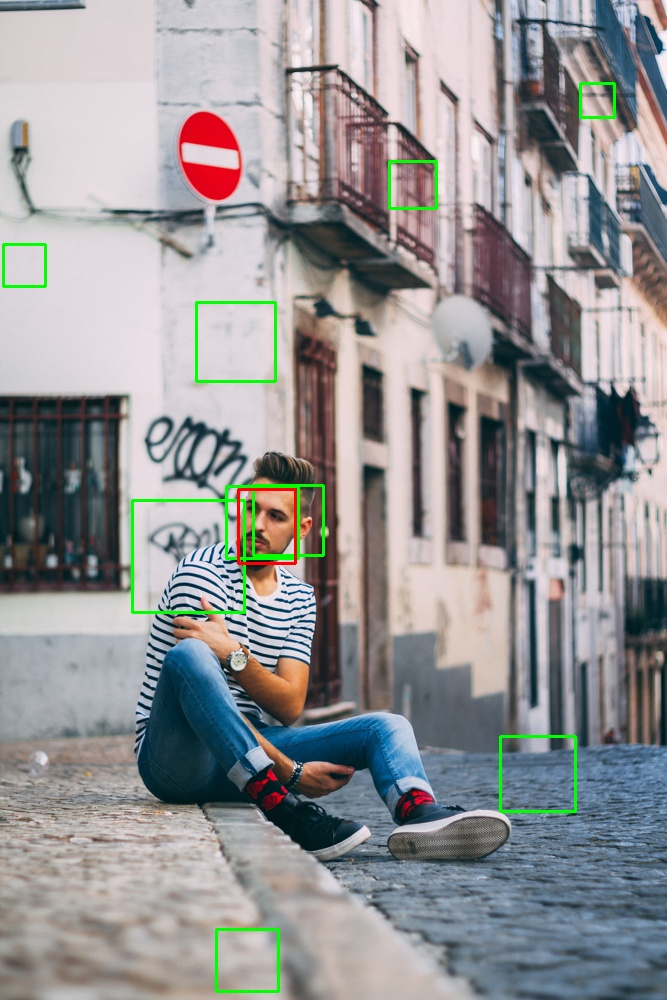
\includegraphics[width = 0.24\textwidth]{images/NoEntry1.jpg}\label{fig:face1}}
  \hfill
  \subfloat[\texttt{NoEntry2.jpg}]{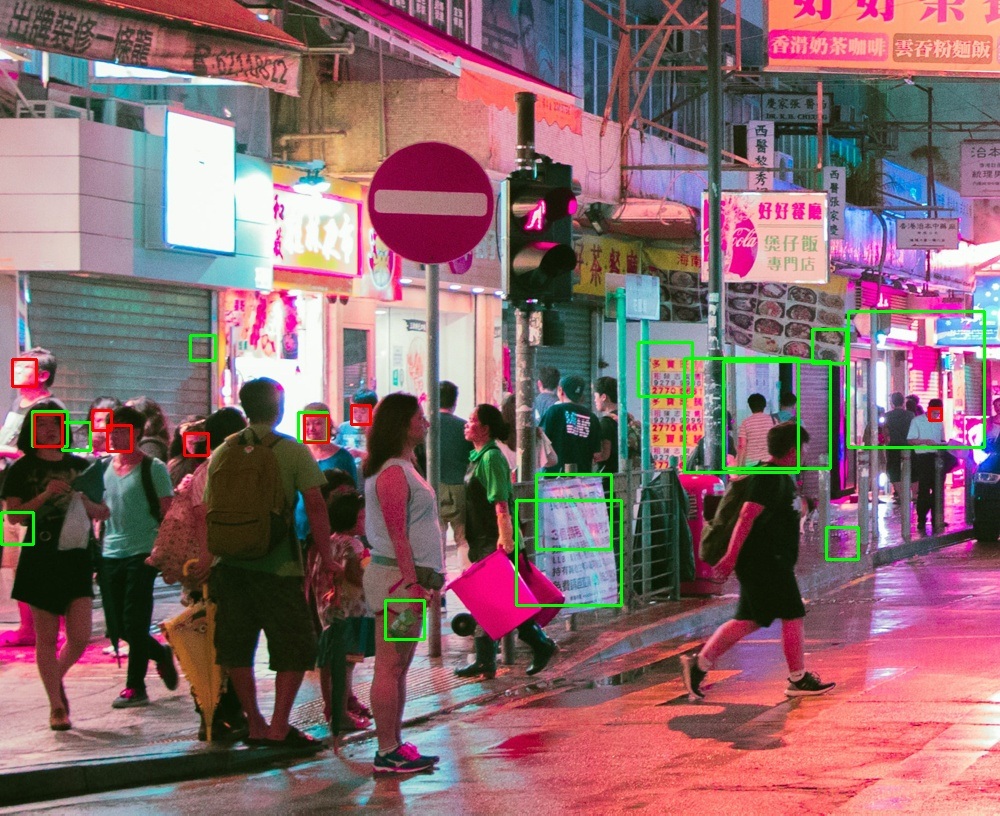
\includegraphics[width = 0.24\textwidth]{images/NoEntry2.jpg}\label{fig:face2}}
  \hfill
  \subfloat[\texttt{NoEntry4.jpg}]{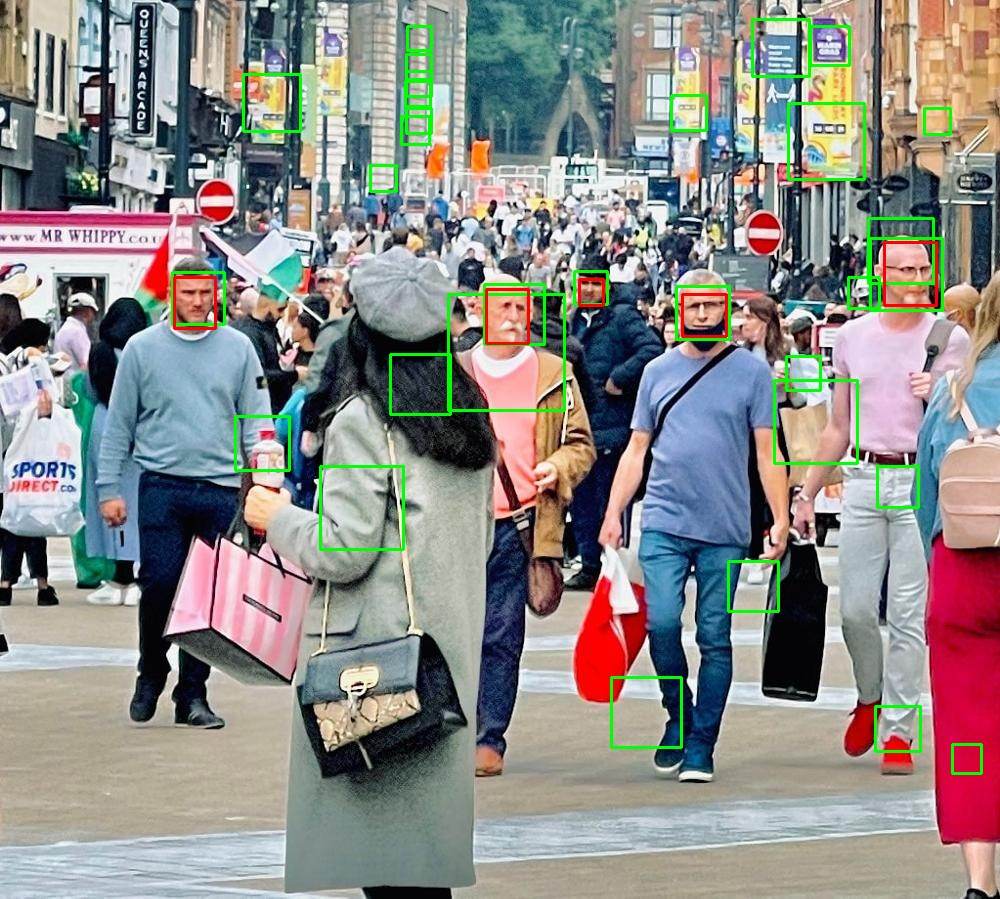
\includegraphics[width = 0.24\textwidth]{images/NoEntry4.jpg}\label{fig:face4}}
  \hfill
  \subfloat[\texttt{NoEntry5.jpg}]{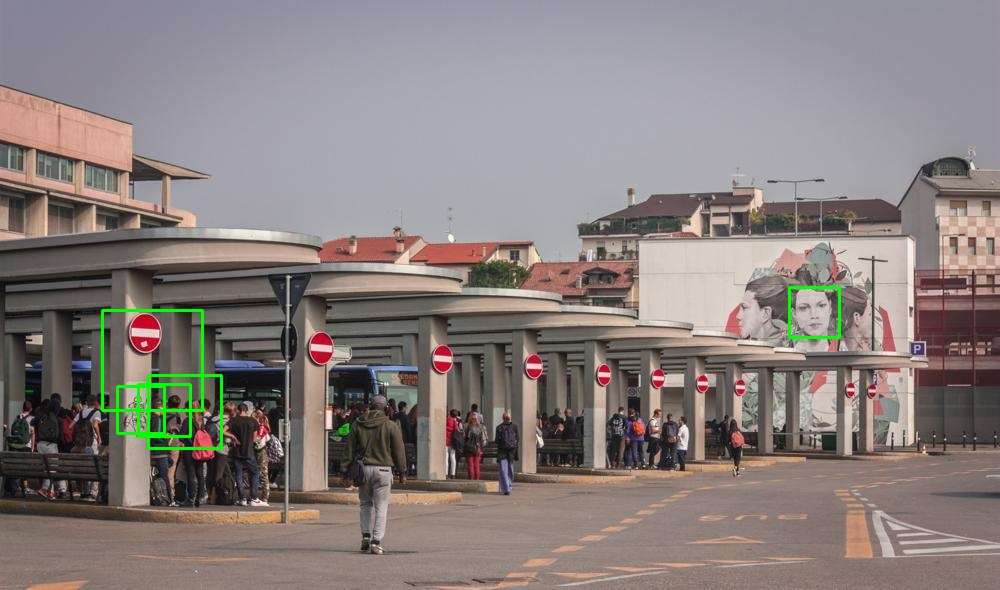
\includegraphics[width = 0.24\textwidth]{images/NoEntry5.jpg}\label{fig:face5}}
  \hfill
  \subfloat[\texttt{NoEntry7.jpg}]{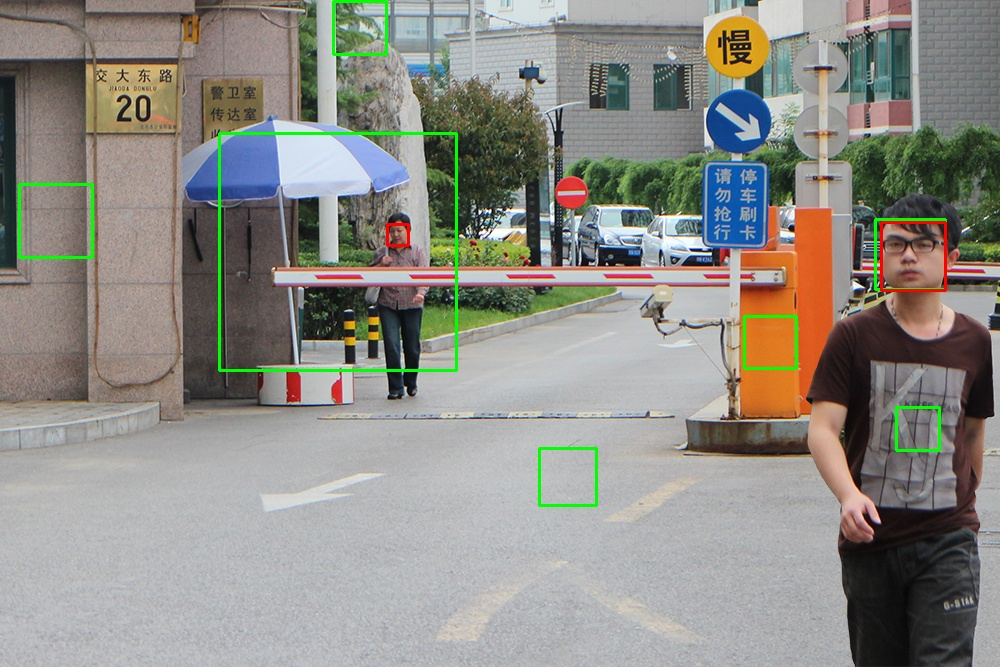
\includegraphics[width = 0.24\textwidth]{images/NoEntry7.jpg}\label{fig:face7}}
  \hfill
  \subfloat[\texttt{NoEntry11.jpg}]{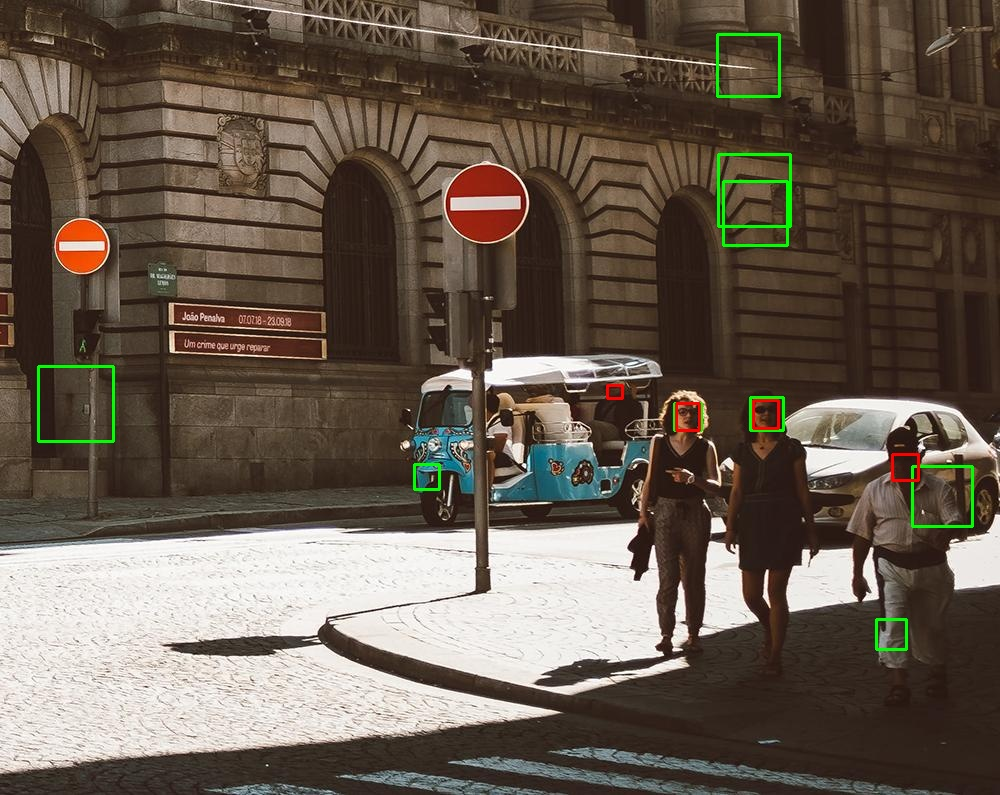
\includegraphics[width = 0.24\textwidth]{images/NoEntry11.jpg}\label{fig:face11}}
  \caption{Six images with the bounding boxes of the ground truths (in red) and actually detected instances (in green) from the frontal face detector}\label{fig:face}
\end{figure}

In object detection tasks, ground truth bounding boxes assist in determining the accuracy of a detection algorithm, and help to visualise how it performs.
Figure \ref{fig:face} displays six images, with their ground truth bounding boxes in red, and the faces detected by \texttt{face.cpp}, which implements the Viola-Jones object detection framework, in green.

For the Viola-Jones frontal face detector, implemented in \texttt{face.cpp}, the ground 

\subsection{Intersection-over-union, true positve rate and F\textsubscript{1} score}

\begin{table}[htbp]
  \begin{center}
  \caption{TPR and F\textsubscript{1} score of the frontal face detector}\label{tab:face}
  \begin{tabular}{l | l l} 
    \hline\hline
    Image&TPR&F\textsubscript{1} score\\
    \hline
    \texttt{NoEntry0.jpg}&Undefined&0.00\\ 
    \texttt{NoEntry1.jpg}&1.00&0.20\\ 
    \texttt{NoEntry2.jpg}&0.25&0.18\\ 
    \texttt{NoEntry3.jpg}&Undefined&Undefined\\ 
    \texttt{NoEntry4.jpg}&1.00&0.28\\ 
    \texttt{NoEntry5.jpg}&Undefined&0.00\\ 
    \texttt{NoEntry6.jpg}&Undefined&0.00\\ 
    \texttt{NoEntry7.jpg}&0.50&0.22\\ 
    \texttt{NoEntry8.jpg}&Undefined&0.00\\ 
    \texttt{NoEntry9.jpg}&Undefined&0.00\\ 
    \texttt{NoEntry10.jpg}&Undefined&0.00\\ 
    \texttt{NoEntry11.jpg}&0.50&0.31\\ 
    \texttt{NoEntry12.jpg}&0.00&0.00\\ 
    \texttt{NoEntry13.jpg}&Undefined&0.00\\ 
    \texttt{NoEntry14.jpg}&Undefined&0.00\\ 
    \texttt{NoEntry15.jpg}&Undefined&0.00\\ 
    \hline
  \end{tabular}
  \end{center}
\end{table} 

In an object detection task, the true positive rate (TPR) is the probability that an object will be positively detected.
However, the first practical difficulty that arises in calculating the TPR is whether or not to define a predicted bounding box as a being a true positive or a false positive.
I opted to define a detected bounding box as being a true positive if it had an intersection-over-union (IoU) value greater than 0.5 with a ground truth bounding box, as this is considered a good score \cite{iou}.
Moreover, for each ground truth bounding box, I only defined the detected bounding box with the largest IoU value as being a true positive if there was more than one intersecting detected bounding box.

In any detection task, TPR can be a flawed metric to use to define how well a given model performs.
This is because, it is possible to achieve a TPR of 100\% by detecting every possible pixel region as being the object being detected, despite having a large number of false positives.
As a result of this, the F\textsubscript{1} score is often used as a measure of a model's accuracy.
F\textsubscript{1} score is the harmonic mean of sensitivity (i.e. TPR) and precision.
Table \ref{tab:face} displays the F\textsubscript{1} score and TPR that `face.cpp' achieved on each of the \texttt{NoEntry\textasteriskcentered.jpg} images

\clearpage

\section{Building and testing my own detector}

\subsection{Training performance}

ROC graph
% \begin{tikzpicture}
% \begin{axis}[]
% \addplot+[
%   only marks,
%   % mark size=2.9pt
% ]
% table[]
% {fpr_tpr.dat};
% \end{axis}
% \end{tikzpicture}

\subsection{Testing performance}

\begin{table}[htbp]
  \begin{center}
  \caption{TPR and F\textsubscript{1} score of Viola-Jones no entry sign detector}\label{tab:vj}
  \begin{tabular}{l | l l} 
    \hline\hline
    Image&TPR&F\textsubscript{1} score\\
    \hline
    \texttt{NoEntry0.jpg}&0.00&0.00\\ 
    \texttt{NoEntry1.jpg}&1.00&0.13\\ 
    \texttt{NoEntry2.jpg}&1.00&0.08\\ 
    \texttt{NoEntry3.jpg}&0.50&0.15\\ 
    \texttt{NoEntry4.jpg}&1.00&0.16\\ 
    \texttt{NoEntry5.jpg}&0.30&0.17\\ 
    \texttt{NoEntry6.jpg}&0.00&0.00\\ 
    \texttt{NoEntry7.jpg}&0.00&0.00\\
    \texttt{NoEntry8.jpg}&0.57&0.62\\ 
    \texttt{NoEntry9.jpg}&0.00&0.00\\ 
    \texttt{NoEntry10.jpg}&0.67&0.33\\ 
    \texttt{NoEntry11.jpg}&0.50&0.11\\ 
    \texttt{NoEntry12.jpg}&0.38&0.21\\ 
    \texttt{NoEntry13.jpg}&0.00&0.00\\ 
    \texttt{NoEntry14.jpg}&0.00&0.00\\ 
    \texttt{NoEntry15.jpg}&0.50&0.40\\ 
    \hdashline
    All images&0.40&0.12\\ 
    \hline
  \end{tabular}
  \end{center}
\end{table} 

\clearpage

\section{Integration with shape detectors}

\begin{figure}[H]
  \vspace{-2em}
  \centering
  \subfloat[\texttt{NoEntry5.jpg} with detected bounding boxes]{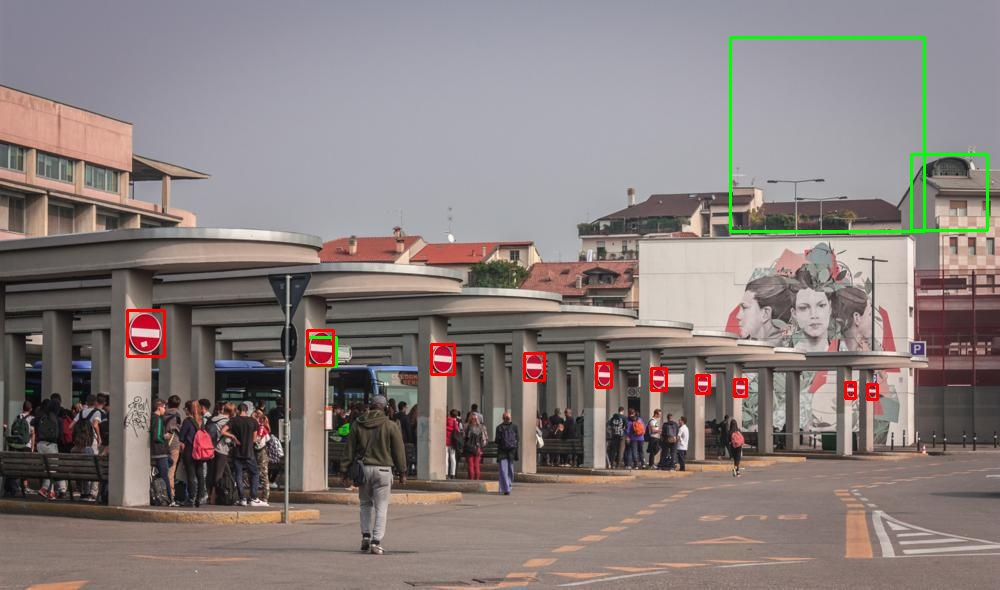
\includegraphics[width = 0.24\textwidth]{images/task_3_5.jpg}}
  \hfill
  \subfloat[\texttt{NoEntry15.jpg} with detected bounding boxes]{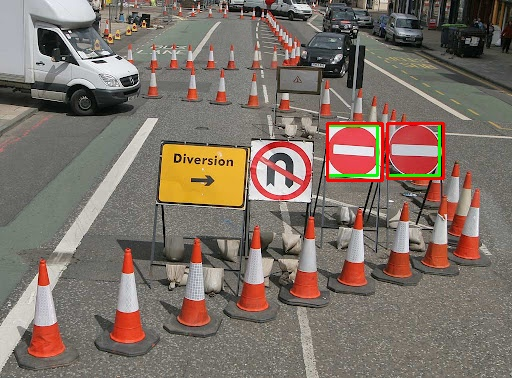
\includegraphics[width = 0.24\textwidth]{images/task_3_15.jpg}}
  \hfill
  \subfloat[\texttt{NoEntry5.jpg} gradient magnitude threshold]{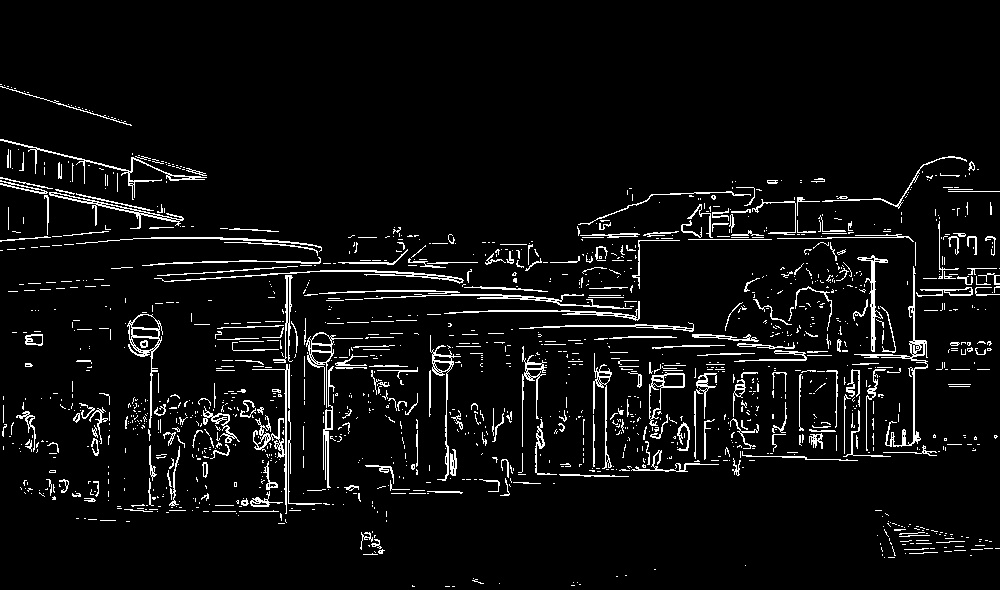
\includegraphics[width = 0.24\textwidth]{images/5_gradient_magnitude_threshold.jpg}}
  \hfill
  \subfloat[\texttt{NoEntry15.jpg} gradient magnitude threshold]{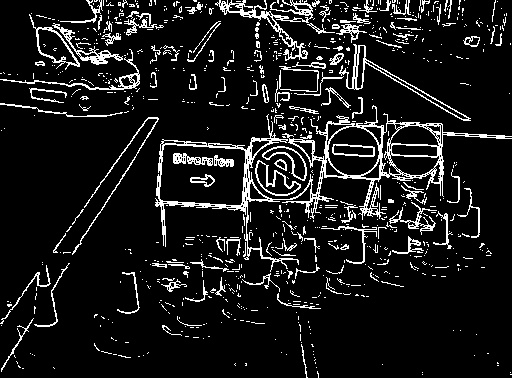
\includegraphics[width = 0.24\textwidth]{images/15_gradient_magnitude_threshold.jpg}}
  \hfill
  \subfloat[\texttt{NoEntry5.jpg} 2D Hough space]{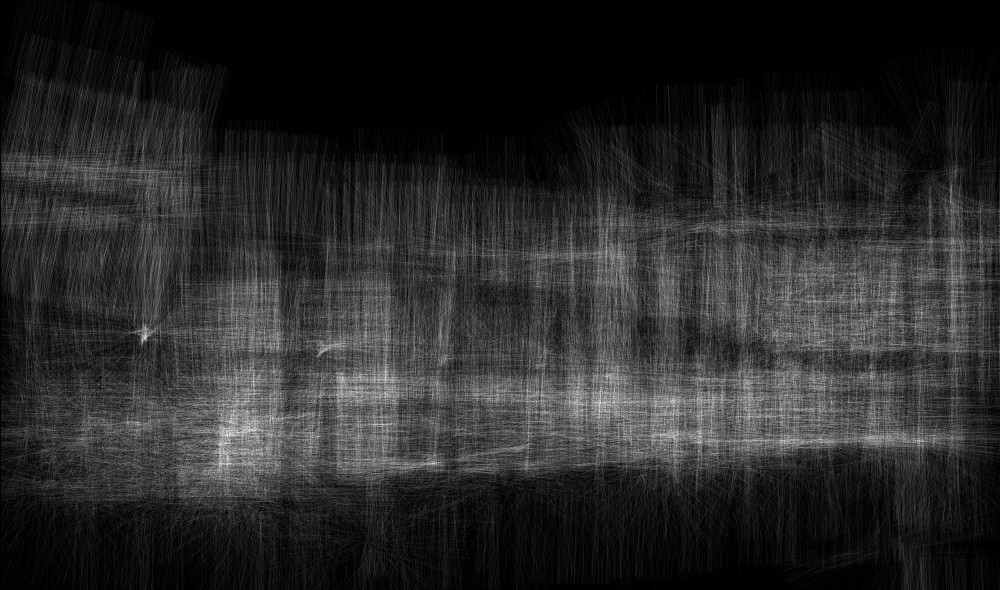
\includegraphics[width = 0.24\textwidth]{images/5_hough_space.jpg}}
  \hfill
  \subfloat[\texttt{NoEntry15.jpg} 2D Hough space]{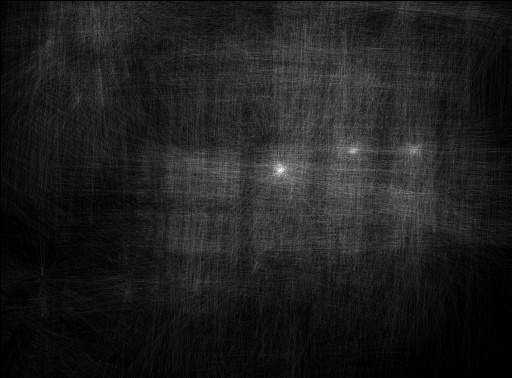
\includegraphics[width = 0.24\textwidth]{images/15_hough_space.jpg}}
  \caption{Two examples of no entry sign images which exhibit the merits and limitations of my implementation}\label{fig:hough_details}
\end{figure}

\subsection{Evaluation}

\begin{table}[htbp]
  \begin{center}
  \caption{TPR and F\textsubscript{1} score of the Viola-Jones integrated with circle Hough transform no entry sign detector and difference with Viola-Jones no entry sign detector results}\label{tab:shape}
  \begin{tabular}{l | l l | l l} 
    \hline\hline
    &\multicolumn{2}{| c |}{Result}&\multicolumn{2}{| c}{Difference}\\
    Image&TPR&F\textsubscript{1} score&TPR&F\textsubscript{1} score\\
    \hline
    \texttt{NoEntry0.jpg}&0.50&0.67&+0.50&+0.67\\
    \texttt{NoEntry1.jpg}&1.00&1.00&$\pm0.00$&+0.87\\
    \texttt{NoEntry2.jpg}&1.00&1.00&$\pm0.00$&+0.92\\
    \texttt{NoEntry3.jpg}&1.00&0.80&+0.50&+0.65\\
    \texttt{NoEntry4.jpg}&1.00&1.00&$\pm0.00$&+0.84\\
    \texttt{NoEntry5.jpg}&0.10&0.15&$-0.20$&$-0.02$\\
    \texttt{NoEntry6.jpg}&0.50&0.67&+0.50&+0.67\\
    \texttt{NoEntry7.jpg}&0.00&0.00&$\pm0.00$&$\pm0.00$\\\
    \texttt{NoEntry8.jpg}&0.43&0.60&$-0.14$&$-0.02$\\
    \texttt{NoEntry9.jpg}&1.00&1.00&+1.00&+1.00\\
    \texttt{NoEntry10.jpg}&0.67&0.80&$\pm0.00$&+0.47\\
    \texttt{NoEntry11.jpg}&0.50&0.67&$\pm0.00$&+0.56\\
    \texttt{NoEntry12.jpg}&0.13&0.22&$-0.25$&+0.01\\
    \texttt{NoEntry13.jpg}&0.00&0.00&$\pm0.00$&$\pm0.00$\\\
    \texttt{NoEntry14.jpg}&0.00&0.00&$\pm0.00$&$\pm0.00$\\\
    \texttt{NoEntry15.jpg}&1.00&1.00&+0.50&+0.60\\
    \hdashline
    All images&0.42&0.56&+0.02&+0.45\\
    \hline
  \end{tabular}
  \end{center}
\end{table} 

Table \ref{tab:shape} displays the TPR and F\textsubscript{1} score of this implementation, as well as the difference compared with the Viola-Jones implementation.
The key merits and shortcomings include:
\begin{itemize}
\itemsep 0em 
\item A vastly improved F\textsubscript{1} score, as a result of only defining no entry signs detected by the Viola-Jones detector as positive if accompanied by a corresponding circle in the circle Hough transform
\item No real improvement to the TPR score, as essentially no extra no entry signs can be detected due to the algorithm used to integrate the two detectors
\end{itemize}

\subsection{Detection pipeline}

Figure \ref{fig:flow} outlines the way I combined evidence in my algorithm.
The rationale behind this was as follows:
\begin{itemize}
\itemsep 0em 
\item The Viola-Jones detector detected approximately 40\% of no entry signs, but had a large number of false positives
\item Upon inspection of the detected bounding boxes, it became clear the Viola-Jones detector appeared to be detecting regions with a light bar horizontally between two dark bars
\item Since no entry signs are circles, we could choose to detect the circles from the circle Hough transform that have an IoU with a Viola-Jones bounding box of greater than 50\%
\end{itemize}

\begin{figure}[htbp]
\centering
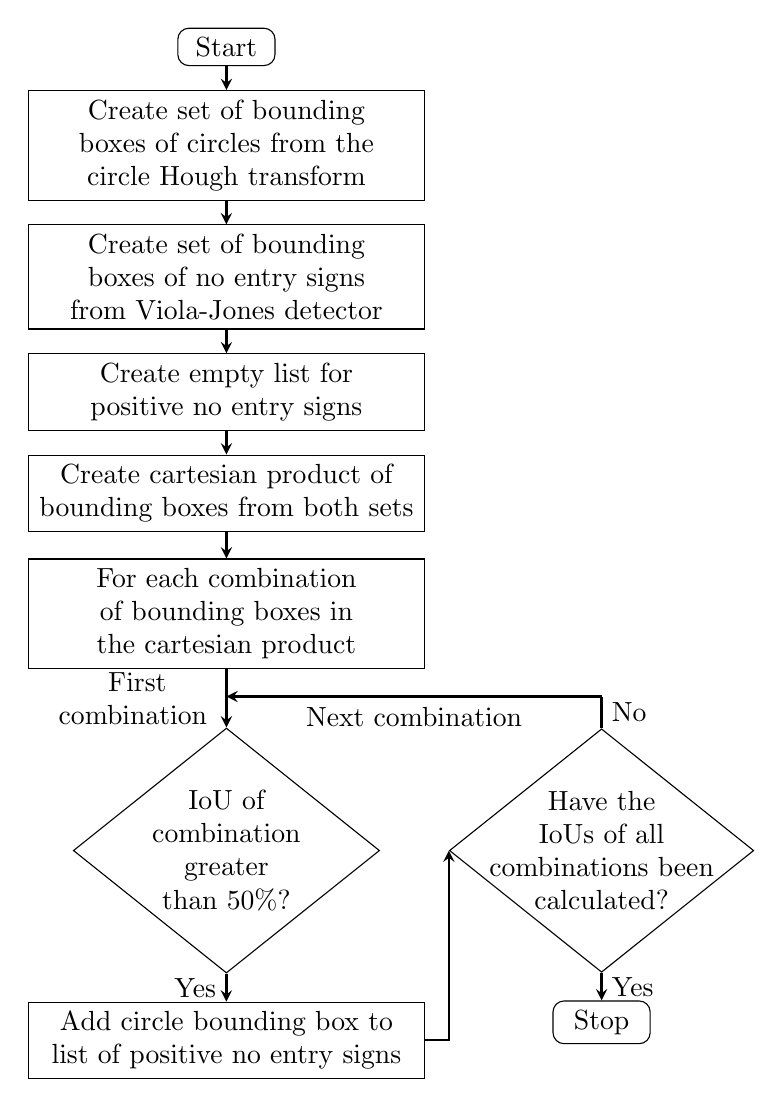
\begin{tikzpicture}[node distance = 1.25cm]
  \node (start) [startstop] {Start};
  \node (hough) [process, below of = start] {Create set of bounding boxes of circles from the circle Hough transform};
  \node (vj) [process, below of = hough, yshift = -1.2em] {Create set of bounding boxes of no entry signs from Viola-Jones detector};
  \node (empty) [process, below of = vj, yshift = -0.6em] {Create empty list for positive no entry signs};
  \node (cartesian) [process, below of = empty, yshift = -0.1em] {Create cartesian product of bounding boxes from both sets};
  \node (for) [process, below of = cartesian, yshift = -0.8em] {For each combination of bounding boxes in the cartesian product};
  \node (iou) [decision, below of = for, yshift = -5em] {IoU of\\combination greater\\than 50\%?};
  \node (list) [process, below of = iou, yshift = -3.3em] {Add circle bounding box to list of positive no entry signs};
  \node (done) [decision, right of = iou, xshift = 10em] {Have the\\IoUs of all\\combinations been\\calculated?};
  \node (stop) [startstop, below of = done, yshift = -2.65em] {Stop};
  \draw [arrow] (start) -- (hough);
  \draw [arrow] (hough) -- (vj);
  \draw [arrow] (vj) -- (empty);
  \draw [arrow] (empty) -- (cartesian);
  \draw [arrow] (cartesian) -- (for);
  \draw [arrow] (for) -- node[anchor = east, text width = 2cm] {\centering First\\combination} (iou);
  \draw [arrow] (iou) -- node[anchor = east] {Yes} (list);
  \draw [arrow] (list.east) -| (done.west);
  \draw let \p1 = (done.north) in [thick,-] (done.north) -- node[anchor = west] {No} (\x1, -8.25);
  \draw let \p1 = (done.north), \p2 = (iou.north) in [arrow] (\x1, -8.25) -- node[anchor = north] {Next combination} (\x2, -8.25);
  \draw [arrow] (done) -- node[anchor = west] {Yes} (stop);
\end{tikzpicture}
\caption{Flow chart detailing my algorithm that integrates Viola-Jones with the circle Hough transform}
\label{fig:flow}
\end{figure}

\clearpage

\section{Improving my detector}



\clearpage

\onecolumn{\printbibliography}
    

\end{document}